\RequirePackage[l2tabu,orthodox]{nag}

% TODO: decide if one-sided/two-sided or whatever
%\documentclass[headsepline,footsepline,footinclude=false,fontsize=11pt,paper=a4,listof=totoc,bibliography=totoc,BCOR=12mm,DIV=12]{scrbook} % two-sided
\documentclass[headsepline,footsepline,footinclude=false,oneside,fontsize=11pt,paper=a4,listof=totoc,bibliography=totoc]{scrbook} % one-sided

\PassOptionsToPackage{table,svgnames,dvipsnames}{xcolor}

\usepackage[utf8]{inputenc}
\usepackage[T1]{fontenc}
\usepackage[sc]{mathpazo}
\usepackage[ngerman]{babel}
\usepackage{upgreek}
\usepackage[autostyle]{csquotes}
\usepackage{siunitx} %SI-units will not be set in italics using this package
\usepackage{icomma} %comma in math-mode

%defining bibliography&citation
\usepackage[
  backend=biber,
  url=false,
  style=authoryear,
  maxbibnames=99,
  maxcitenames=1,
  firstinits=true,
  doi=false,
  isbn=false,
  sorting=nyt,
  uniquename=init]{biblatex} % TODO: BIBLIOGRAPHYSETTINGS
\DefineBibliographyStrings{ngerman}{andothers={et\ al\adddot}} % "u.a." zu "et al." 
\DefineBibliographyStrings{ngerman}{and={\&}} % "und" zu "&"

\usepackage{graphicx}
\usepackage{lstautogobble}
\usepackage{booktabs}
\usepackage{tabularx} %adjusting tablewidth to textdwidth
\usepackage{multirow}
\usepackage{scrhack}
\usepackage[final]{microtype}
\usepackage{caption}
\usepackage[hidelinks]{hyperref} % hidelinks removes colored boxes around references and links
\usepackage[toc,nonumberlist,acronym]{glossaries}

\usepackage{float} %Position erzwingen 
\usepackage{setspace} %anderthalbzeiliger Zeilenabstand
%\onehalfspacing
%\usepackage{hyperref}

\usepackage{glossaries}
\usepackage{glossary-mcols}
\bibliography{bibliography/library}
\setkomafont{disposition}{\normalfont\bfseries} % use serif font for headings
\linespread{1.05} % adjust line spread for mathpazo font

% Settings for glossaries
\renewcommand{\glsnamefont}[1]{\normalfont\bfseries #1} % use serif font for glossary entry titles
\makeglossaries{}
\renewcommand*{\glspostdescription}{} % Removes dots at the end of each entry.
%graphicspath
\graphicspath{ {./figures/} }
%Anderthalbzeilen
\onehalfspacing




% Basic information for cover & title page
\newcommand*{\getUniversity}{Technische Universität München}
\newcommand*{\getFaculty}{Fakultät für Medizin}
\newcommand*{\getTitle}{Oligomerization of $\upbeta_2$-Adrenergic Receptors}
\newcommand*{\getTitleGer}{Oligomerisierung von $\upbeta_2$-Adrenorezeptoren}
\newcommand*{\getAuthor}{Stephan Skawran}
\newcommand*{\getDoctype}{Dissertation zur Erlangung des akademischen Titels Dr. med.}
\newcommand*{\getSupervisor}{Prof. Dr. Dr. Stefan Engelhardt}
\newcommand*{\getAdvisor}{Dr. Andrea Ahles}
\newcommand*{\getSubmissionDate}{TODO: Submission date}
\newcommand*{\getSubmissionLocation}{München}


\begin{document}

\input{pages/cover}

\frontmatter{}

\begin{titlepage}
{\par \centering

  \vspace{40mm}
  \includegraphics[width=40mm]{logos/tum}

  \vspace{5mm}
  {\huge\MakeUppercase{\getFaculty{}}}\\
    
  \vspace{5mm}
  {\large\MakeUppercase{\getInstitute{}}}\\

  
\par}

  \vspace{10mm}
  \large{ Vollständiger Abdruck der von der Fakultät für Medizin der Technischen Universität München zur Erlangung des akademischen Grades eines Dr. med. genehmigten Dissertation.}

  \vspace{10mm}
{\par \centering
  {\huge\bfseries \getTitleGer{}}\\
  \vspace{5mm}
  {\LARGE \getAuthor{}}
  \vspace{10mm}
  
  \begin{tabular}{l l}
    \large{Vorsitzender:}                    & \large{\getSupervisor{}} \\
    \large{Prüfer der Dissertation:}        & \large{1.} \\
                                    & \large{2.} \\
                                    & \large{3.} \\
    \end{tabular}
\\
\par}

\vspace {10mm}

\large{Die Dissertation wurde am \getSubmissionDate{} bei der Technischen Universität München eingereicht und durch die Fakultät für Medizin am \getSubmissionDate{} angenommen}. 

\vspace {10mm}
  \centering
  \includegraphics[width=20mm]{logos/faculty}
\end{titlepage}

\thispagestyle{empty}
\vspace*{0.8\textheight}
\noindent
Ich erkläre an Eides statt, dass ich diese, bei der Fakultät für Medizin der TUM zur Promotionsprüfung vorgelegte Arbeit ohne sonstige Hilfe erstellt und bei der Abfassung nur die gemäß § 6 Abs. 6 und 7 Satz 2 angegebenen Hilfsmittel benutzt habe.

\vspace{15mm}
\noindent
\getSubmissionLocation{}, \getSubmissionDate{} \hspace{5cm} \getAuthor{}

\cleardoublepage{}

\addcontentsline{toc}{chapter}{Danksagung}
\thispagestyle{empty}

\vspace*{2cm}

\begin{center}
{\usekomafont{section} Danksagung}
\end{center}

\vspace{1cm}

%TODO: Acknowledgments

\cleardoublepage{}

\glsaddall{} % add all defined terms to glossary, even if not referenced in text

%{name}{Abkürzung}{Langform}
\newacronym{zb}{z.B.}{zum Beispiel}
\newacronym{dmso}{DMSO}{Dimethylsulfoxid}
\newacronym{beta2}{$\beta_2$AR}{$\beta_2$-Adrenorezeptor}
\newacronym{ici}{ICI}{ICI-118,551}
\newacronym{pbs}{PBS}{Dulbecco's Phosphate Buffered Saline}
\newacronym{trfret}{trFRET}{time resolved Fluorescence Resonance Energy Transfer}
\newacronym{snap}{SNAP-tag}{Markenname des auf der O\textsuperscript{6}-Alkylguanin-DNA-Alkyltransferase basierenden Proteinlabelingsystems}
\newacronym{clip}{CLIP-tag}{s. SNAP-tag}
\newacronym{mis}{MIS}{Membraninsertionssequenz}
\newacronym{iso}{Iso}{Isoproterenol}
\newacronym{epi}{Epi}{Epinephrin}
\newacronym{bg}{BG}{Benzyl-Guanin}
\newacronym{lumi4}{Lumi4}{Markenname des trFRET-kompatiblen Terbium-Cryptats, das in vorliegender Arbeit als Donorfluorophor verwendet wurde}

\printglossary[title=Verzeichnis der Abkürzungen,type=\acronymtype]

\microtypesetup{protrusion=false}
\tableofcontents{}
\microtypesetup{protrusion=true}

\mainmatter{}

\chapter{Introduction}\label{chapter:introduction}

\section{Firstsection}
Citation test \parencite{Ahles2011}.
\gls{zb}
Ich habe viele Ideen, 
\gls{dmso} \gls{dmso}



\subsection{Subsection}
See~\autoref{fig:sample}.

\begin{figure}[htsb]
  \centering
  \includegraphics{logos/tum}
  \caption[Example figure]{An example for a figure.}\label{fig:sample}
\end{figure}

\section{Section}

See~\autoref{tab:sample}

\begin{table}[htsb]
  \caption[Example table]{An example for a simple table.}\label{tab:sample}
  \centering
  \begin{tabular}{l l l l}
    \toprule
      A & B & C & D \\
    \midrule
      1 & 2 & 1 & 2 \\
      2 & 3 & 2 & 3 \\
    \bottomrule
  \end{tabular}
\end{table}
 %Beispielseiten

\chapter{Einleitung}\label{chapter:einleitung}
%TODO: ADRB2, durchgehend; Skalen; Deckblatt

\section{G-Protein-gekoppelte Rezeptoren (GPCR)}
\label{generalGPCR}
G-Protein-gekoppelte Rezeptoren (GPCRs) stellen die größte Familie der Membranproteine dar. Sie vermitteln zelluläre Antworten auf Hormone und Neurotransmitter, bilden die Rezeptoren des olfaktorischen Systems und können sogar Photonen in zelluläre Signale umsetzen \parencite{Rosenbaum2009}. Allein für das olfaktorische System sind hunderte strukturell verwandter GPCRs bekannt. Damit bilden Moleküle, die GPCRs zum Ziel haben heute die Gruppe der am meisten verwendeten Medikamente \parencite{Pierce2002}.

Alle GPCRs besitzen sieben hydrophobe alpha-helikale Transmembransegmente (7TM-Rezeptoren). Das Aminoende (N-Terminus) ist extrazellulär lokalisiert, das Carboxyende (C-Terminus) intrazellulär. Dazwischen liegen alternierend intra- und extrazelluläre Schleifen. 

Bei beeindruckender funktioneller Diversität lassen sich die GPCRs aufgrund struktureller Homologien in fünf Familien unterteilen \parencite{Fredriksson2003}: Rhodopsin- (Klasse A), Sekretin- (Klasse B), Glutamat- (Klasse C), Adhäsions- (Klasse D) und Frizzled/Taste-Rezeptoren (Klasse E).
Die bei weitem größte unter ihnen bilden die rhodopsinverwandten Rezeptoren (dem "`Lichtrezeptor"' ähnliche Rezeptoren), zu denen auch der in dieser Arbeit näher untersuchte $\beta_2$-adrenerge Rezeptor (ADRB2) gehört.
\subsection{Signaltransduktion}

GPCRs sind in der Lage, stimulatorische (Gs) und inhibitorische guaninnukleotidbindende Proteine (G-Proteine) zu binden, die zu unterschiedlichen Signalkaskaden führen (s. Abb. \ref{fig:gpcr}): 

\begin{figure}[htbp]
	\centering
    \includegraphics[width=1.0\textwidth]{fig_gpcr.pdf}
    \caption{\textbf{Signaltransduktion eines GPCRs am Beispiel des ADRB2 ($\boldsymbol\beta_2$AR) aus \cite{Rosenbaum2009}}} 
    \label{fig:gpcr}
\end{figure}

Anhand der Funktion des ADRB2 kann die klassische Funktion eines GPCRs illustriert werden: Nach Bindung der natürlichen Agonisten Adrenalin oder Noradrenalin wird die stimulatorische Untereinheit eines heterotrimeren G-Protein aktiviert (G$\alpha$S). Diese führt zur Stimulation der Adenylatzyklase und damit zur Produktion von zyklischem AMP (cAMP). Das akkumulierte cAMP wiederum aktiviert die cAMP-abhängige Proteinkinase A (PKA), die Proteine phosphoryliert und inaktiviert, die für die Kontraktion glatter Muskelzellen verantwortlich sind (L-Typ-Kalziumkanäle) \parencite{Hoffman1982}. 

Die Aktivierung des ADRB2 führt daneben zur Phosphorylierung durch die G-Protein-gekoppelte Rezeptorkinase (GRK). Die Phosphorylierung ermöglicht die Bindung des Proteins Arrestin, das seinerseits als regulatorisches und Signalprotein fungiert. Es deaktiviert den GPCR und führt über Clathrinpits zur endozytotischen Internalisierung des Rezeptors (s. Abschnitt \ref{internalization}), der danach entweder zur Membran recycled oder in Lysosomen degradiert wird. 

Daneben bedingt Arrestin die Aktivierung extrazellulärer signalregulierter Kinasen (ERK 1,2). Diese wiederum regulieren über MAP (mitogen-activated-pathway)-Kinasen die Genexpression.

\section{Adrenerge Rezeptoren}
\subsection{Das $\beta$-adrenerge System}
Die Klasse der adrenergen Rezeptoren umfasst $\alpha$- und $\beta$-adrenerge Rezeptoren. Diese wiederum lassen sich in drei $\alpha_1$-Subtypen ($\alpha_{1A}$, $\alpha_{1B}$, $\alpha_{1D}$), drei $\alpha_2$-Subtypen ($\alpha_{2A}$, $\alpha_{2B}$, $\alpha_{2C}$) sowie in die beiden $\beta$-Subtypen $\beta_1$ und den in dieser Arbeit betrachteten $\beta_2$-Rezeptor unterteilen (\url{http://www.guidetopharmacology.org}).

\subsection{Polymorphismen der $\beta$-adrenergen Rezeptoren}
\subsection{Rezeptorinternalisierung}
\label{internalization}
Gleichzeitig zur Entdeckung, dass durch Agonisten der $\beta$-adrenergen Rezeptoren ein zellulärer  Signalprozess in Gang gesetzt wird, konnten Veränderungen der Rezeptorendichte auf der Membran gefunden werden \parencite{Chuang1979}. 

\section{Oligomerisierung G-Protein-gekoppelter Rezeptoren}
\subsection{Homo- und Heterooligomerisierung G-Protein-gekoppelter Rezeptoren}
Die klassische Annahme, GPCRs würden als monomere Proteine funktionieren, konnte durch eine große Zahl unterschiedlicher Studien widerlegt werden. Tatsächlich sind nach zahlreichen BRET- und FRET-gestützten Untersuchungen mittlerweile sowohl Hetero- als auch als Homodimere einer Vielzahl von GPCRs bekannt (\cite{Khelashvili2010}, \url{http://www.gpcr-okb.org}).

Als Reaktion auf die stetig wachsende Informationen über Rezeptoroligomerisierung veröffentlichte die International Union of Basic and Clinical Pharmacology (IUPHAR) drei Kriterien, von denen mindestens zwei erfüllt sein sollen, um die physiologische Relevanz der Oligomere einordnen zu können \parencite{Pin2007}. Die drei Kriterien umfassen:
\begin{enumerate}
\item Den Nachweis der physischen Interaktion der am Oligomer beteiligten Rezeptoren in nativem Gewebe oder primären Zellen. Dabei wird hinreichende methodische Sicherheit gefordert: Bloße Co-Immunopräzipitationsstudien genügen beispielsweise nicht für den überzeugenden Nachweis physischer Interaktion.
\item Funktionelle oligomerspezifische Besonderheiten wie positive oder negative allosterische Interaktion oder auch den Nachweis eines oligomerspezifischen Liganden (s. Abschnitt \ref{drugs}). Auch der Nachweis einer spezifisch durch den Oligomer modifizierten Signalskaskade kann an dieser Stelle stehen.
\item Validierung des Rezeptoroligomers in-vivo mittels beispielsweise Knock-Out-Mäusen oder RNAi-basierten Methoden - unter der Voraussetzung, dass in heterologen Expressionssystemen bereits hinreichende Relevanz bestätigt werden konnte. 

\end{enumerate}

Zwar ist die Existenz der Rezeptoroligomere in vielen Fällen akzeptiert, doch führt die Bewertung ihrer funktionellen Bedeutung weiter zu kontroversen Diskussionen - etwa weil sich die meisten Untersuchungen heterologer Expressionssysteme bedient haben, die, um Heterooligomere zu untersuchen Rezeptoren exprimierten, die in-vivo nicht gemeinsam exprimiert werden. Zum anderen ist weiter in Diskussion, welche Untereinheiten der Rezeptoren tatsächlich das Interface der beobachteten Rezeptoroligomere bilden \parencite{Terrillon2004}. 

Ebenso bleibt Gegenstand der Diskussion, wie viele Rezeptoren in einem Oligomer gruppiert sind. Häufiger taucht die These auf, Dimere seien die vorherrschende stöchiometrische Einheit \parencite{Dorsch2009}, erst mit steigender Expressionstärke ergäben sich höhergradige Oligomere \parencite{Calebiro2013}. Gleiches konnte für den GABA\textsubscript{B}-Rezeptor beobachtet werden \parencite{Maurel2008, Comps-agrar2011}. Untersuchungen, die sich der Fluorescence-Correlation-Spectroscopy (FCS) und Photon-Counting-Histogram (PCH) bedienen, deuten ebenfalls darauf hin, dass Dimere bei mehreren GPCRs die funktionelle Einheit bilden \parencite{Herrick-Davis2013}. In der vorliegenden Arbeit wird der Begriff "`Oligomere"' bei weiter nicht vollständig geklärter Stöchiometrie bevorzugt, da die wahrscheinliche Dimer-Konfiguration einen Spezialfall des allgemeineren Begriffes darstellt.
\\ \\
Rezeptoroligomere haben eine Reihe denkbarer Implikationen. Fünf postulierte und beobachtete Rollen der Rezeptoroligomerisierung sind in Abbildung \ref{fig:lifecycle} illustriert:

\begin{figure}[htbp]
	\centering
    \includegraphics[width=1.0\textwidth]{fig_lifecycle.pdf}
    \caption{\textbf{Rolle der Rezeptoroligomerisierung (aus \cite{Terrillon2004}):} 1 Rezeptorreifung; 2 Dynamische Regulierung der Oligomerisierung durch Ligandenbindung; 3 Heterodimerisierung von Rezeptoren bedingt positiv- oder negativ-kooperative Ligandenbindung; 4 verstärkte und inhibierte Signaltransduktion als Folge der Rezeptoroligomerisierung; 5 Heterooligomerisierung ruft möglicherweise Rezeptorinternalisierung schon bei Aktivierung nur eines Protomers hervor beziehungsweise blockiert ein endozytoseresistenter Protomer die Internalisierung seines gekoppelten Rezeptors im Heterooligomer} 
    \label{fig:lifecycle}
\end{figure}
\begin{itemize}
\item So sind Biosynthese und korrekte posttranslationale Modifikationen im endoplasmatischen Retikulum (ER) möglicherweise Voraussetzung für Integration in die Zellmembran \parencite{Salahpour2004}. Wurden GPCRs mit einem Retentions-Signal versehen, das den Export aus dem Endoplasmatischen Retikulum verhinderte, bedingte dies die Retention des untersuchten Heterooligomers \parencite{Zhu1998, Lee2000, Issafras2002, Floyd2003}.
\item Im Falle des Heterooligomers aus $\mu$- und $\delta$-Opioid-Rezeptoren wurde beobachtet, dass die Bindung eines für den einen Rezeptor spezifischen Liganden über Beeinflussung der Rezeptorkonfirmation die Affinität für den Agonisten des anderen verstärkt \parencite{Gomes2004}. Ein Phänomen, das als positive Kooperativität bezeichnet wird.
\item Auf der Ebene der durch G-Proteine vermittelten Signalkaskade (s. Abschnitt \ref{generalGPCR}) konnte für die Dopaminrezeptoren D1 und D2 im Heterooligomer veränderte Bindungseigenschaften gegenüber dem Gq/11-Protein und somit veränderte Signaleigenschaften gemessen werden \parencite{Rashid2007}.
\item Schließlich konnte gezeigt werden, dass Rezeptorinternalisierung eines Protomers im Fall von Heterooligomeren effektiv auch zur Internalisierung des anderen führen, beziehungsweise diese verhindern kann \parencite{Hillion2002, Milligan2010, Ward2011}. 
\end{itemize}

\subsection{Physiologische Relevanz von Rezeptoroligomeren}
In einer Reihe von Pathologien konnte eine Bedeutung von Rezeptoroligomerisierung im Zusammenhang mit den oben genannten Mechanismen identifiziert werden:
\\ \\
In der Asthmatherapie spielen beispielsweise Agonisten des ADRB2 als Bronchodilatatoren eine führende Rolle. In einer Publikation von \cite{McGraw2006} wurde ein Cross-Talk zwischen dem Prostanoid-Rezeptor EP1 (EP1R) und dem ADRB2 gezeigt: Prostaglandin E2 (PGE2) führte zu verstärkter Dimerisierung des EP1R und des ADRB2 - mit geringerer cAMP-Produktion als Zeichen verminderter ADRB2-Aktivierung.

Bei Patienten mit Major-Depression wurde der Anteil oligomerisierter D1- und D2-Rezeptoren in post-mortem-Studien mittels Co-Immunopräzipitation signifikant erhöht gegenüber gesunden Probanden gemessen \parencite{Pei2010}. Möglicherweise können in Zukunft Medikamente, die die Oligomerisierung der beiden Rezeptoren beeinflussen, therapeutische Bedeutung für die Depression gewinnen. 

In mehreren Untersuchungen, unter anderem mit bivalenten Liganden (s. Abschnitt \ref{drugs}), wurde dem Heterooligomer aus $\delta$- und$\mu$-OR negative Kooperativität in-vivo beigemessen \parencite{Daniels2005, Lenard2007, He2011}. Ähnlich wie bei beim Dopaminrezeptor im Falle der Depression könnte Beeinflussung der Oligomerisierung von pharmakologischer Relevanz werden.
\\ \\
Weitere physiologisch bedeutsame Konstrukte konnten bei der Parkinson-Erkrankung \parencite{Tanganelli2004, Fuxe2003, Fuxe2005} sowie bei Prä-Eklampsie (Hypertonie) \parencite{AbdAlla2001} gefunden werden.

\subsection{Rezeptoroligomere als zukünftiges drug-target}
\label{drugs}
\parencite{George2002, Hiller2013, Ferre2014}
%TODO: incorporate George 2002, Ferré 2014

\section{Methoden zur Untersuchung der Oligomerisierung von Rezeptoren}
\subsection{Überblick}
Es existieren eine Vielzahl von Methoden, die zum Nachweis von Rezeptoroligomerisierung verwendet worden sind. 

\subsubsection {Co-Immunopräzipitation}
Eine der am häufigsten verwendeten Methoden stellt die Co-Immunopräzipitation dar \parencite{Hebert1996, Jordan1999, Hillion2002, Park2004}. In der einfachsten Variante mit einem Protein-Epitop-tag und dem passenden spezifischen Antikörper war aufgefallen, dass die untersuchten Rezeptoren jeweils in den Banden ganzzahliger Vielfacher des Molekulargewichts liefen. Der Vermutung, es könnte sich um Oligomere handeln, liegt nahe. Allerdings konnte so nicht ausgeschlossen werden, dass es sich um unspezifische Rezeptor-Protein-Aggregate handelte. Genauer gelang der Nachweis mithilfe zweier Protein-Epitop-tags und zwei spezifischen Antikörpern. So konnten untersuchte Rezeptoren erst immunpräzipitiert und anschließend mit dem zweiten Antikörper geblottet werden.

\subsubsection{Kristallstrukturen oligomerisierter Rezeptoren}
Eine direkte Nachweismöglichkeit oligomerisierter Rezeptoren bietet die aufwändige Gewinnung der Kristallstruktur der Rezeptoren. Im Falle des CXCR4-Chemokin-Rezeptors und der Opioid-Rezeptor-Subtypen $\mu$OR und $\kappa$OR konnten in den Kristallstrukturen strikte Rezeptordimere beobachtet werden \parencite{Wu2010, Manglik2012, Wu2012}. Die mit dieser Methode identifizierten Oligomerisierungsinterfaces waren für die jeweiligen Rezeptoren unterschiedlich lokalisiert und werden in Zukunft Gegenstand weiterer Analysen werden.

\subsubsection{Fluoreszenz-basierte Methoden}
Fluoreszenz-basierte Methoden zur Analyse der Oligomerstruktur von GPCRs bedienen sich dem Resonanzenergietransfer (RET) zwischen biolumineszenten oder synthetischen Fluorophoren. In Abschnitt \ref{ret} sind die Methoden genauer dargestellt.

\subsubsection{Funktionelle Untersuchungen}

\subsection{BRET \& FRET zur Analyse oligomerisierter Rezeptoren}
\label{ret}
Am häufigsten kommen \gls{bret} und \gls{fret} zum Einsatz. Bei BRET-basierten Analysen werden Fusionsproteine generiert, die C-terminal über ein biolumineszentes Protein, beispielsweise Renilla reniformis Luciferase (Rluc) als Donor und fluoreszente Proteine wie YFP als Akzeptor.

%TODO:RET-acro
\subsection{Proteinlabeling mit dem SNAP-tag}
Zur spezifischen Adressierung von Proteinen wie den GPCRs existieren eine Reihe unterschiedlicher Systeme. Neben Verfahren, die sich auf strukturell große Antikörper stützen können tag-Systeme mit intrinsischer Aktivität verwendet werden, um spezifische kovalente mit den gewünschten Proteinuntereinheiten zu katalysieren \parencite{Gautier2008}.
\subsection{time-resolved FRET}

\section{Zielsetzung dieser Arbeit}
\chapter{Material \& Methoden}\label{chapter:materialmethoden}

\chapter{Ergebnisse} \label{chapter:ergebnisse}
\section{Generierung von $\beta_2$-Adrenorezeptoren mit dem SNAP-tag} \label{klonierung}
Zur Untersuchung der Oligomerisierung des \gls{beta2} wurde der Rezeptor so modifiziert, dass er über eine extrazelluläre Komponente verfügte, die Untersuchungen mit fluoreszierenden Substraten ermöglichte. Der SNAP-tag ermöglicht über seine O\textsuperscript{6}-Alkylguanin-DNA-Alkyltransferase-Aktivität die kovalente Bindung nahezu beliebiger Moleküle \parencite{Gronemeyer2006}. Die gewünschten Fluorophore müssen dazu eine O\textsuperscript{6}-Benzylguanin oder O\textsuperscript{6}-Alkylguanin-Gruppe tragen. Viele Fluorophore, darunter trFRET-kompatible, sind kommerziell verfügbar. Die Funktionsweise ist in Abbildung \ref{fig:snap-tag} dargestellt

\begin{figure}[htp]
    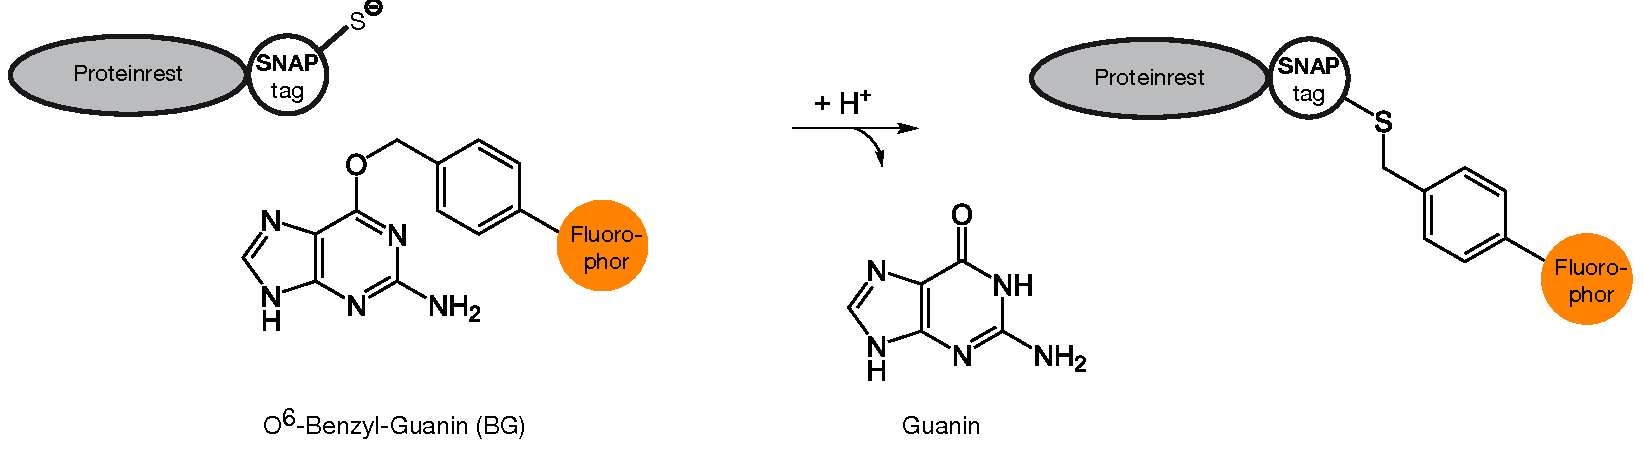
\includegraphics[width=0.97\textwidth]{SNAP-tag.pdf}
    \caption{\textbf{Funktionsweise des SNAP-tag}}
    \label{fig:snap-tag}
\end{figure}

Darauf basierend wurden Vektoren kloniert, die den \gls{beta2} trugen, der N-terminal über den SNAP-tag verfügte. 
\\ \\
Mittels Fluoreszenzmikroskopie konnte initial gezeigt werden, dass mit der N-terminalen Modifikation des \gls{beta2} keine Membranexpression des \gls{beta2} mehr erfolgte (s. Abb. \ref{fig:stainsnap} in \ref{snapmikro}). Infolgedessen wurde weiter N-terminal eine Proteinsequenz zur Membraninsertion verwendet, die zur zufriedenstellenden Expression des \gls{beta2} führte. 
\\ \\
In Abbildung \ref{fig:klonierung} sind schematisch die Klonierungsstrategien zu den final verwendeten Vektoren dargestellt. Es wurden Expressionsvektoren erzeugt, die die SNAP-getaggten natürlich vorkommenden Varianten Arg16 und Gly16 des \gls{beta2} exprimierten.
\\ \\ 
Darüber hinaus wurden zwei weitere Expressionssysteme generiert: Ein Vektor, der den \gls{beta2} mit dem SNAP-tag im zweiten extrazellulären Loop trug, sowie einen weiteren, der die in der Literatur als dimerisierungsdefizient beschriebene Variante Tyr284 \parencite{Salahpour2004} enthielt.
\\ \\
Für zukünftige Anwendung wurden außerdem analog Vektoren kloniert, die den mit dem CLIP-tag versehenen \gls{beta2} trugen (nicht dargestellt). 

\begin{figure}[htp]
    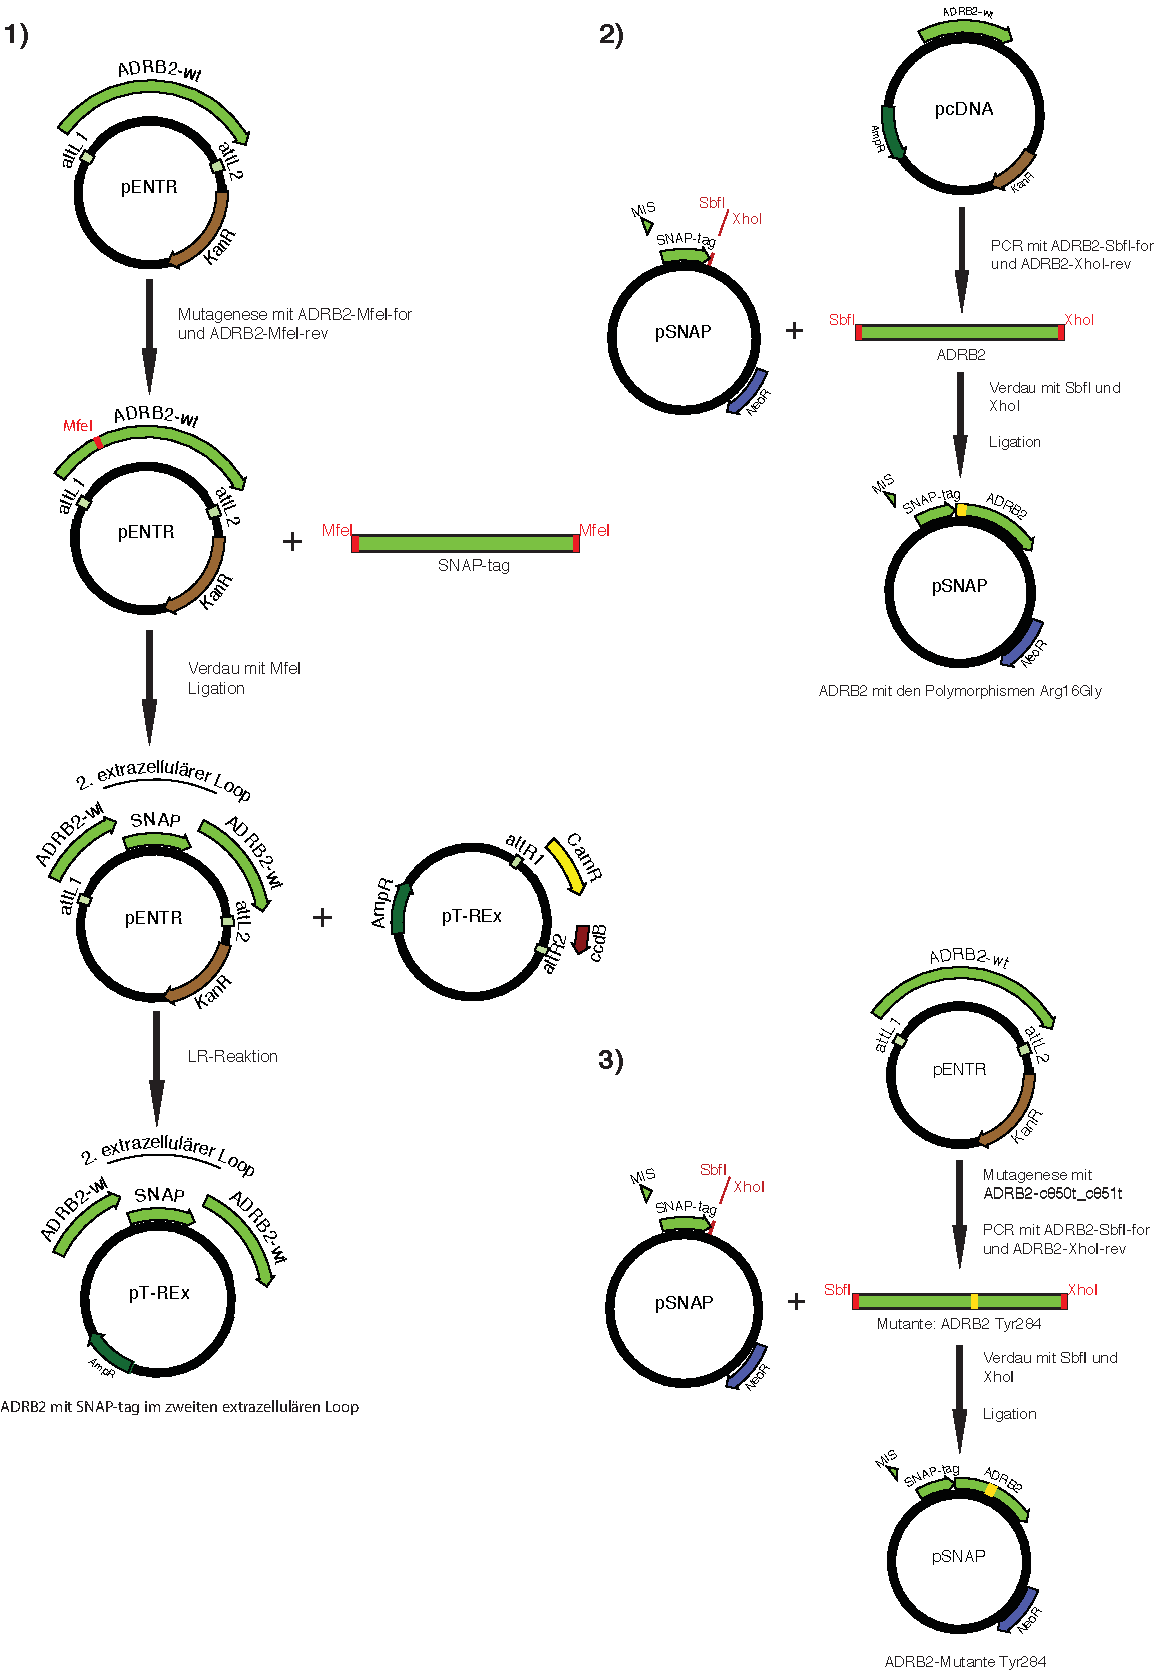
\includegraphics[width=0.97\textwidth]{cloning.pdf}
    \caption{\textbf{Klonierungsstrategien}: \textbf{1)} Generierung eines Expressionsvektors mit dem SNAP-tag im zweiten extrazellulären Loop des \gls{beta2}; \textbf{2)} SNAP-tag am N-Terminus des \gls{beta2}; \textbf{3)} SNAP-tag am N-Terminus der dimerisierungsdefizienten Mutante des \gls{beta2}}
    \label{fig:klonierung}
\end{figure}

\section{Fluoreszenzmikroskopie des \gls{beta2} mit dem SNAP-tag} \label{snapmikro}

Die Charakterisierung der Oligomerisierung des \gls{beta2} zunächst außer Acht gelassen, wurden zuerst Fluoreszenzfärbungen mit SNAP-Substraten durchgeführt. Dabei sollte geprüft werden, ob der mit dem SNAP-tag versehene Rezeptor korrekt in die Zellmembran integriert wird, bzw. noch trivialer, ob die Transfektion mit zufriedenstellender Effizienz gelungen war.

Wie in \ref{klonierung} beschrieben, konnten erfolgreich Vektoren erzeugt werden, die den mit dem SNAP-tag versehenen \gls{beta2} trugen. Diese Plasmide konnten in die HeLa- und HEK293-Zelllinien transient transfiziert werden.

\begin{figure}[htp]
    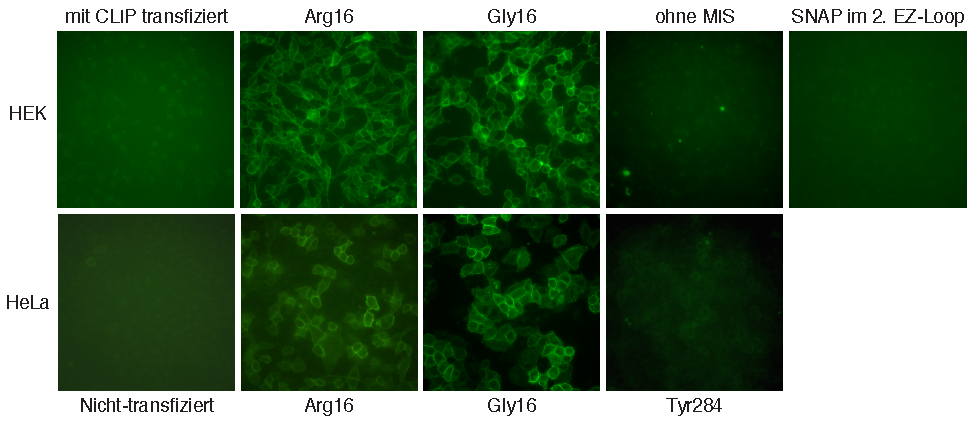
\includegraphics[width=1.0\textwidth]{snap_fluormikro.pdf}
    \caption{\textbf{Fluoreszenzfärbung mit SNAP-Substraten:} transient exprimierende HEK293- und stabile HeLa-Zellen.}
    \label{fig:stainsnap}
\end{figure}

Zunächst wurden direkt nach der Transfektion in HEK293-Zellen mit BG-Alexa-488 SNAP-basierte Fluoreszenzfärbungen durchgeführt. Dabei zeigten sich die in Abbildung \ref{fig:stainsnap} in der mit HEK gekennzeichneten Zeile dargestellten Expressionsmuster: Als Negativkontrolle dienten entweder nicht transfizierte Zellen oder Zellen, die mit dem \gls{beta2} transfiziert worden waren, der den CLIP-tag trug. Für den Arg16Gly-Polymorphismus zeigte sich in beiden Fällen ein deutliches Membranexpressionsmuster mit vernachlässigbarem Hintergrundsignal. Für die Variante des Vektors, der N-terminal vor dem SNAP-tag kein Membraninsertionssignal enthielt, war keine Membranfärbung nachweisbar. Auch die Variante des \gls{beta2}, die den SNAP-tag im zweiten extrazellulären Loop trug, war fluoreszenzmikroskopisch kein Membranexpressionsmuster erkennbar. Die Tyr284-Variante, wurde in HeLa-Zellen transfiziert. Dort war keine Membranfärbung erkennbar.
\\ \\
HEK293-Zellen eigneten sich aufgrund ihrer geringen Adhärenz nicht für die weiteren Versuchsreihen, die allesamt häufiges Waschen benötigten. Somit wurden stabile Zelllinien nur mit den stärker adhärenten HeLa-Zellen generiert. Diese zeigten in der Fluoreszenzmikroskopie eine den HEK293-Zellen vergleichbare Membranexpression. Die Ergebnisse sind in Abbildung \ref{fig:stainsnap} dargestellt. Sowohl bei der Arg16- als auch bei der Gly16-Variante des \gls{beta2} war eine klare lineare Membranfärbung feststellbar.

\section{Oligomerisierung des \gls{beta2} mit SNAP-tag}
Zur Analyse der Oligomerisierung des \gls{beta2} wurde der in der Einleitung beschriebene trFRET-Ansatz verwendet. Dazu wurden zuerst mit trFRET kompatible Fluorophore, die an Substrate des SNAP-tag gekoppelt waren, in unterschiedlichen Versuchsreihen zur Untersuchung der prinzipiellen Oligomerisierung des modifizierten \gls{beta2} eingesetzt. In den in Abschnitt \ref{ligandenfret} vorgestellten Ergebnissen konnten dann fluoreszierende Liganden des unveränderten \gls{beta2} in analogen Versuchsreihen die Oligomerisierung des Rezeptors zeigen.

\subsection{\gls{trfret} mit SNAP-Substraten}
Mit Hilfe der trFRET-Methode konnte die räumliche Interaktion von Molekülen es \gls{beta2} nachgewiesen werden. Dazu wurde in einem ersten Schritt die optimale Konzentration des Donorfluorophors bestimmt. Darauf konnte eine räumliche Interaktion gemessen werden. In einem letzten Schritt wurde gezeigt, dass diese spezifisch war.

\subsubsection{Bestimmung der Sättigungskinetik der SNAP-Substrate}
Zur optimalen Einstellung der Konzentrationen der verwendeten SNAP-Substrate wurden Sättigungsassays durchgeführt. Dazu wurden steigende Konzentrationen des mit dem Donorfluorophor Lumi4 verbundenen SNAP-Substrats (Lumi4-BG) mit Zellen inkubiert, die den SNAP-getaggten \gls{beta2} trugen. Diese Zellen waren zuvor fluoreszenzmikroskopisch auf ihre Expression untersucht worden. Als Negativkontrolle und zur Abschätzung unspezifischer Bindung des SNAP-Substrates dienten nicht-transfizierte Zellen. Über die Messung der Intensität der Fluoreszenz des Donorfluorophores bei 620nm konnte auf die Sättigung der SNAP-tags Rückschluss gezogen werden. Das Ergebnis ist in Abbildung \ref{fig:lumi4binding} dargestellt.
\\ \\
\begin{figure}[htbp]
	\centering
    \includegraphics[width=0.6\textwidth]{lumi4binding.pdf}
    \caption{\textbf{Bindungskinetik des Lumi4-Donorfluorophors}}
    \label{fig:lumi4binding}
\end{figure}
Über steigenden Konzentrationen des SNAP-Substrates zeigte sich ein sigmoider Intensitätsverlauf, der bei spezifischer sättigbarer Bindung zu erwarten ist. Die unspezifische Bindung erwies sich als gering. Für die weitere Analyse waren mehrere Bedingungen zu optimieren: Zum einen sollte die Konzentration der SNAP-Substrate gering gehalten werden, um nicht-spezifische Bindung vernachlässigen zu können. Zum anderen war für eine zufriedenstellende signal-to-noise-ratio eine ausreichend hohe Konzentration zu wählen.

Diese Bedingung waren am besten bei der etwa halbmaximal sättigenden Konzentration des SNAP-Substrates gegeben. Für die Analyse der spezifischen Interaktion der SNAP-getaggten Rezeptoren wurde daher die Konzentration des Donor-Substrates auf 10\si{\nano M} festgelegt.

\subsubsection{Räumliche Interaktion des SNAP-getaggten \gls{beta2}}
\begin{figure}[htbp]
	\centering
    \includegraphics[width=0.5\textwidth]{bell.pdf}
    \caption{\textbf{Maximierung des FRET-Signals}}
    \label{fig:bell}
\end{figure}
    
\subsubsection{Nachweis der spezifischen Interaktion zwischen Rezeptoroligomeren}

\subsection{Einfluss der Stimulation mit Liganden des \gls{beta2} auf seine Oligomerisierung}

\subsection{Einfluss der Glycosylierung auf die Oligomerisierung des \gls{beta2}}

\section{\gls{trfret} mit fluoreszierenden Liganden des \gls{beta2}}
\label{ligandenfret}


\chapter{Diskussion}\label{chapter:diskussion}

\chapter{Zusammenfassung}\label{chapter:zusammenfassung}

Entgegen dem klassischen Paradigma, die Gruppe der G-Protein-gekoppelten Rezeptoren sei strukturell auf Einzeleinheiten (Monomeren) basiert, geht man heute vom Vorhandensein konstitutiver Rezeptoroligomeren als erstem Signaltransduktor bei der zellulären Signalisierung aus. Zwar existierten bislang  eine Reihe von Untersuchungsmethoden, die diese These stützten, doch fehlten zur substantiellen Validierung noch Systeme, die unter in-vivo-Bedingungen spezifische Evidenz liefern können.

Mit dieser Arbeit konnte mittels einer auf tr-FRET basierenden Methode speziell die Oligomerisierung des \gls{beta2} untersucht werden. Dazu wurden zunächst mehrere Untersuchungsmethoden etabliert und validiert. 

Zuerst konnten unter Verwendung des SNAP-tag geeignete Expressionssysteme generiert werden, die die kovalente Bindung tr-FRET-kompatibler Fluorophore erlaubten. Mit dieser Methode gelang der Nachweis von Rezeptoroligomeren und die Untersuchung von modulierenden Faktoren. Es konnte gezeigt werden, dass der zellmembrangebundene ADRB2 Oligomere mindestens der Größenordnung zwei bildet.

 Weiter zeigte die Bindung von den ADRB2 adressierenden Agonisten, nicht jedoch die von Antagonisten oder inversen Agonisten einen signifikanten Signalanstieg des tr-FRET-Signals zwischen oligomerisierten Rezeptoren. Es ist davon auszugehen, dass die Anhebung des Signals nicht mit einer denkbaren Änderung der Anzahl der sich in einem Rezeptoroligomer befindlichen Monomere in Verbindung gebracht werden kann, sondern mit N-terminalen Konformationsänderungen der untersuchten Rezeptorspezies im Rahmen von Internalisierung unter Agonistenstimulation einhergeht. 
 
 Durch die ausbleibende Signaländerung bei Stimulation mit einem inversen Agonisten konnte dieser als in Bezug auf die Rezeptoroligomerisierung neutral eingestuft und für die folgende Ligandensynthese priorisiert werden. 
 
 Weiter konnte gezeigt werden, dass weder den bekannten Polymorphismen noch der Rezeptorglykosylierung des ADRB2 im Zusammenhang mit der Oligomerisierung eine Rolle zukommt.

 Nach dem prinzipiellen Nachweis der Oligomerisierung konnte der nicht-modifizierte \gls{beta2} mittels fluoreszierender Liganden weiter charakterisiert werden. Dazu wurden geeignete Liganden zur Synthese in Auftrag gegeben. Mit diesen bislang nicht verfügbaren invers antagonistischen Rezeptorliganden höchster Spezifität konnte auf membrangebundene Rezeptoroligomere auf transfizierten HEK-Zellen analog zu den zuvor untersuchten geschlossen werden. 
 
 Damit konnte die prinzipielle Eignung eines tr-FRET basierten Ansatzes im Falle des ADRB2 auch für native Zellen gezeigt werden. Dem Institut steht somit fortan ein leistungsfähiges Instrumentarium für weitere Untersuchungen zur Verfügung.
 
 Mit der Etablierung der Methoden ergeben sich für zukünftige Anwendungen essentielle Grundlagen sowie die Möglichkeit des Transfers auf andere Rezeptoren.


\appendix{}


\microtypesetup{protrusion=false}
\listoffigures{}
\listoftables{}
\microtypesetup{protrusion=true}
\printbibliography{}

\end{document}